\documentclass[twocolumn]{aastex62}

\newcommand{\vdag}{(v)^\dagger}
\newcommand\aastex{AAS\TeX}
\newcommand\latex{La\TeX}
\usepackage{amsmath}
\usepackage{physics}
\usepackage{hyperref}
\usepackage{natbib}
\usepackage[T1]{fontenc}
\usepackage[english]{babel}
\usepackage[utf8]{inputenc}
\usepackage{wasysym}

\begin{document}

\title{\Large AST5220-Milestone I: The Background Cosmology}

\author{Nils-Ole Stutzer}

\begin{abstract}

\end{abstract}

\section{Introduction} \label{sec:Intro}
In order to discribe the universes evolution the first, perhaps most fundamental
part, is to discribe its large scale dynamics. Thus in this project we will define some consepts and quantities used to discribe the
large scale dynamics of the universe as a whole, since the Big Bang untill
today, the so-called Background Cosmology. The main equation used for this is
the Friedmann equation. Furthermore, we will study how the different components
of the matter-energy content of the universe evolves and how the paticle horizon
evolves as the universe expands.


\section{Method} \label{sec:Method}
\subsection{Consepts and Quantities}
Before starting on how to solve for the evolution of the universe as a whole, we
start introducing some consepts and quantities.
Because we know from previously conducted cosmological experiments (KILDER) that
the universe is nearly flat, we will here only consider the case of a flat
universe filled with a homogenous and isotropically distributed matter-energy
content. The latter of which is called the cosmological principal. Doing theis
the invariant line-element is given by the Friedmann–Lemaître–Robertson–Walker
metric (FLRW metric) 
\begin{align}
    ds^2 &= -c^2dt^2 + a^2(t)(dr^2 + r^2(d\theta^2 +\sin^2\theta d\phi^2))\\
    & = a^2(t)(-d\eta^2 + dr^2 + r^2(d\theta^2 +\sin^2\theta d\phi^2)),
\end{align}
where $a(t)$ and $eta$ denote the scale factor and the conformal time
respectively. The scale factor quantifies the expansion of the universe, being a
translation factor between proper (physical) and comoving distances. For
convinience we introduce the log-scale facor $x \equiv \log a$ (base $e$),
because we will consider a wide range of universe scales. The universe scale
today at $t = t_0$ is  normalized to $a(t = t_0) = a_0 = 1$, or in log-scale $x_0 = 0$. The
conformal time is the total time a photon is able to travle since the Big Bang
at $t = 0$
until a time $t$, and is thus also a measure of cosmic time. It is thus equivalent to the particle horizon scale of the
universe at any given time, and we will here define it by a ordinary
differential equation  (ODE)
\begin{align}
    \dv{\eta}{t} = \dv{\eta}{a}\dv{a}{t} =  \frac{c}{a},
\end{align} 
which we can rewrite into 
\begin{align}
    \dv{\eta}{a} = \frac{c}{a^2 H} = \frac{c}{a\mathcal{H}}.
    \label{eq:conf_time}
\end{align}
Here $H(a)\equiv \frac{\dot{a}}{a}$ is the Hubble parameter measuring the
expansion rate of the universe. We define the scaled Hubble parameter
$\mathcal{H}(a) \equiv aH(a)$. 

The Hubble parameter is given by the Friedmann
equation
\begin{align}
    H = H_0 \sqrt{(\Omega_{b,0} + \Omega_{CDM,0})a^{-3} + \Omega_{r,0} a^{-4} + \Omega_{\Lambda,0}},
    \label{eq:friedmann}
\end{align} 
where $H_0 = 100 h$ $\mathrm{km s^{-1} Mpc^{-1}}$ is the Hubble parameter today
(Hubble constant, and the dimensionless Hubble parameter is usually set to $h = 0.7$) and the $\Omega_{x,0}$'s are the matter-energy density parameters
today defined as $\Omega_{x,0}\equiv \frac{\rho_{x,0}}{\rho_{c,0}}$ for a energy
component $x$. The critical density $\rho_c\equiv \frac{3H^2}{8\pi G}$, is the
density needed in order to have a flat universe, and is today equal to
$\rho_{c,0}\equiv\frac{3H_0^2}{8\pi G}$.  

In order to know how much each component of the matter-energy content of the
universe contributes to the total energy content, we can compute the
matter-energy density of each component. This is done when solving the
continuity equation 
\begin{align}
    \dot{\rho} + 3H(\rho + P) = 0,
\end{align}
having the solution 
\begin{align}
    \rho_{x} = \rho_{x,0} a^{-3(1+\omega)},
\end{align}
where $\rho_x$, $\rho_{x,0}$ and $\omega = P/\rho$ are the density at a given
time $a(t)$, the density today and the equation of state (EOS) parameter for a
matter energy component $x$, respectively. For pressureless fluids like baryons
and cold dark matter (CDM) $\omega = 0$, for relativistic particles like
radiation $\omega = 1/3$ and for dark energy (the cosmological constant) $\omega
= -1$. 

It is, however, more convinient to instead compute the energy density parameters
given as 
$\Omega_x(a) = \rho_x / \rho_c$ at any time. Writing out these we get for a
component $x$ that 
\begin{align}
    \Omega_x &= \frac{\rho_x}{\rho_c} = \frac{\rho_{x,0}a^{-3(1+\omega)} 8\pi G}{3 H^2} \\
   &= \frac{\rho_{x,0}}{\rho_{c,0}/H_0^2} \frac{a^{-3(1+\omega)}}{H^2} \\ 
   &= \frac{\Omega_{x,0}}{(H/H_0)^2} a^{-3(1+\omega)}.
\end{align}

Inserting the respective EOS parameters we get that the energy density parameter
for baryonic matter, CDM, radiation and dark energy ($\Lambda$)
at any given universe scale $a$ is given as

\begin{align}
    \Omega_b(a) &= \frac{\Omega_{b,0}}{a^3 (H/H_0)^2}\\
    \Omega_{CDM}(a) &= \frac{\Omega_{CDM,0}}{a^3 (H/H_0)^2}\\
    \Omega_r(a) &= \frac{\Omega_{r,0}}{a^4 (H/H_0)^2}\\
    \Omega_\Lambda(a) &= \frac{\Omega_{\Lambda,0}}{(H/H_0)^2},
\end{align}
where we have neglected the curvature parameter $\Omega_k$, sometimes included in
the energy-density parameters, as we only consider a flat universe here. Also we
have not included the neutrinos on the calculations. 

We know that at any given time these density parameters must sum to 1, as they
respectively represent the fraction of matter-energy contribution to the total
content of the universe. This can for instance be seen from the Friedmann
equation (\ref{eq:friedmann}), when inserting the scale facor today $a_0 = 1$,
we must recover $H = H_0$ or else it would not make sence. Thus the density
parameters today sum to 1, and for any other time one can simply sum the above
density parameters and check wheter they sum to unity.
The values of the density parameters today are well known from cosmological
surveyes like Planck, and we will here use the values provided by (CALLIN 2006)
here. These can be found in Table \ref{tab:params}

\begin{deluxetable}{rc}
	%\tablewidth{0pt}
	\tablecaption{Table showing the energy density parameter values at the current time. \label{tab:params}}
	%\tablecomments{}
	
	\tablecolumns{2}
	\tablehead{$x$ & $\Omega_{x,0}$}
	\startdata
	$CDM$  &  0.224  \\
	$b$ & $0.046$  \\
	$\Lambda$ & $0.72995$   \\
	$r$ & $5.042\cdot 10^{-5}$  
	\enddata
\end{deluxetable}

Note that the radiation density parameter is given by 
\begin{align}
    \Omega_r = 2\frac{\pi^2}{30} \frac{(k_B T_{CMB})^4}{\hbar^3 + c^5}\frac{8\pi G}{3H_0^2},
\end{align}
where the temperature of the Cosmic Micowave Background (CMB) $T_{CMB} =
2.7255\mathrm{K}$, and the Boltzmann constant, reduced Planck constant and the speed of
light take their regular SI values in our calculations.

\subsection{Implementation}

We want to know how the universe as a whole evolves from the Big Bang until
today. To do that we want to compute the evolution of the regular and the scaled
Hubble parameters as a function of the log-scale factor $x$ (as we consider a wide
range of scales $a$). This is simply done by generating an array of $x$ values
and compute the Hubble parameters from the Friedmann equation
and the scaled Hubble parameter by simply multiplying the
regular Hubble parameter by the scale factor $a = e^x$. One can simply use the
Friedmann equation on the form (\ref{eq:friedmann}), only having to change the
scale factors $a$ to log-scale factors $a = e^x$. Next, one can compute the
density parameters from their definition given in the previous subsection, by
simply also exchanging the scale factor with an exponential of the log-scale
factor. 

Further, we want to compute the conformal time (particle horizon scale). This is
done by simply solving the ODE given in equation (\ref{eq:conf_time}) using the
\texttt{ODESolver} (C++) module cindly provided by Hans A. Winther. We use initial
conditions $\eta(x) = 0$, as the horizon was very small at early times. We
cannot use $a = 0$ here, though, as this results in a singularity. We thus use
$a = 10^{-8}$, corresponding to $x \approx -18.42$, to represent the scale at
early times. We let the siumulation run until $x = 2$ so as to see what happens
beyond the current age. We solve the ODE using 1000 points and save them to a
file together will the corresponding other quantities (the $\Omega$'s, $H$ etc.)
After solving for $\eta(x)$ we have a discrete set of conformal times and
corresponding log-scale factors. To get a more continous representation, we then
perfrom a cubic spline interpolation, so as to enable computation of the
conformal time between the previously found discrete values. This is done using
the \texttt{Spline} modulde cindly provided by Hans A. Winther.

To illustrate the evolution of the large scale universe we now can plot the
density parameters as a function of the log-scale factor $x$, as well as the
horizon scale, the regular and scaled Hubble parameters as functions of $x$.
Also we plot the Hubble parameter as a function of redshift $z$, being another
measure of time. It is related to the scale factor by $a^{-1} = 1 + z$, and
measures how much a wavelength of light is streached as light travels through an
expanding universe.

\section{Results/Discussion}\label{sec:Results}
The conformal time (horizon scale) as well as the Hubble
and scaled Hubble parameters as functions of $x$ ($z$ and $a$) can be seen in
Figure \ref{fig:Eta}. As one can see the horizon scale stayes very small for a
long while, from early times until $x \approx -7$, then starting to grow
exponentially and finally starting to flatten out towards the end of the
simulated period.
(DISKUTER)

The expansion rate quantified by the scaled Hubble parameter $\mathcal{H}(x) =
aH(x)$ is also seen in Figure \ref{fig:Eta}. We can clearly see from its shape
in which era of the universe we are in. At early times, when the universe was
radiation domminated the scaled Hubble parameter $\mathcal{H} \propto a^{-1}$.
When matter (baryons and CDM) eventually started dominating, the expansion rate
scaled differently; $\mathcal{H}\propto a^{-0.5}$, having a somewhat shallower
slope compared to the expansion rate at radiation domminance. This transion
seems to happen at $x\sim -7$, coinsiding roughly with the sudden growth of
$\eta$, as seen for the change in slope of $\mathcal{H}$. Finally we see the
transition from a decelerating universe, to an accelerating one. The expanding
universe halts, as seen by the extremum of $\mathcal{H}$, after which the curve
turns upwards. This corresponds to the era of dark matter, where the universe
gradually turns to an exponential expansion rate. This hypothisis is further
supported by the fact that the regular Hubble parameter seen in the bottom left
pannel of Figure \ref{fig:Eta} becomes almost constant (in the log-log) after
crossing into the era of dark energy. This is easily seen from the Friedmann
equation, assuming that the other densty parameters are negligable. Another
notworthy thing is that the Hubble parameter seems to hit its known current
value (see red dot in Figure \ref{fig:Eta}) pretty well, putting further
evidence on that the solving of the equations are done correctly. The plot in the lower right
pannel of Figure \ref{fig:Eta} tells the same story as the lower left one,
however, it is nice to see the redshift (scale factor) dependence of the Hubble
parameter directly.

\begin{figure*}
    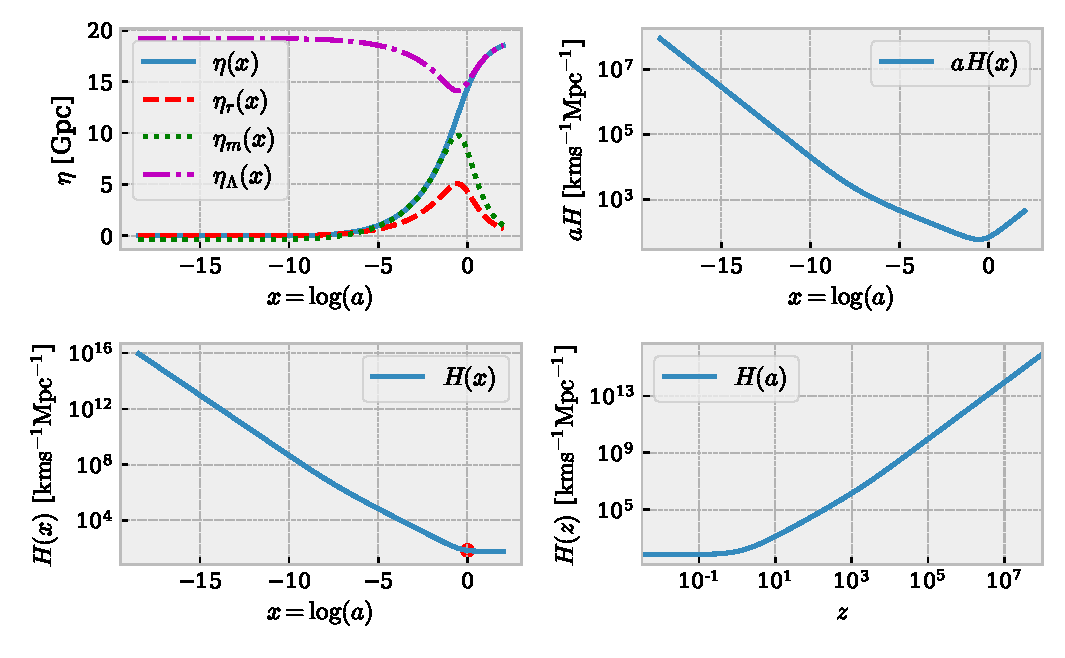
\includegraphics[scale=1]{Figures/Eta_&_H_of_x.pdf}
    \caption{\textbf{Upper left:} The figure shows the conformal time $\eta$(horizon scale) in Gpc as a function of the log-scale factor $x$. \textbf{Upper right:} The figure shows the scaled Hubble parameter (expansion rate $\dot{a}$) as a function of the log-scale factor $x$. \textbf{Lower pannels:} Here the Hubble parameter $H$ is shown as a function of the log-scale facor $x$ (\textbf{left pannel}) and as a function of the scale factor $a$ and the redshift $z$ (\textbf{right pannel}), in addithon to a red dot illustrating the Hubble parameters value today. Note that the Hubble parameter as a function of the redshift is only plotted from early times until today, while the remaining plots go a bit further.}
    \label{fig:Eta}
\end{figure*}



\begin{figure*}
    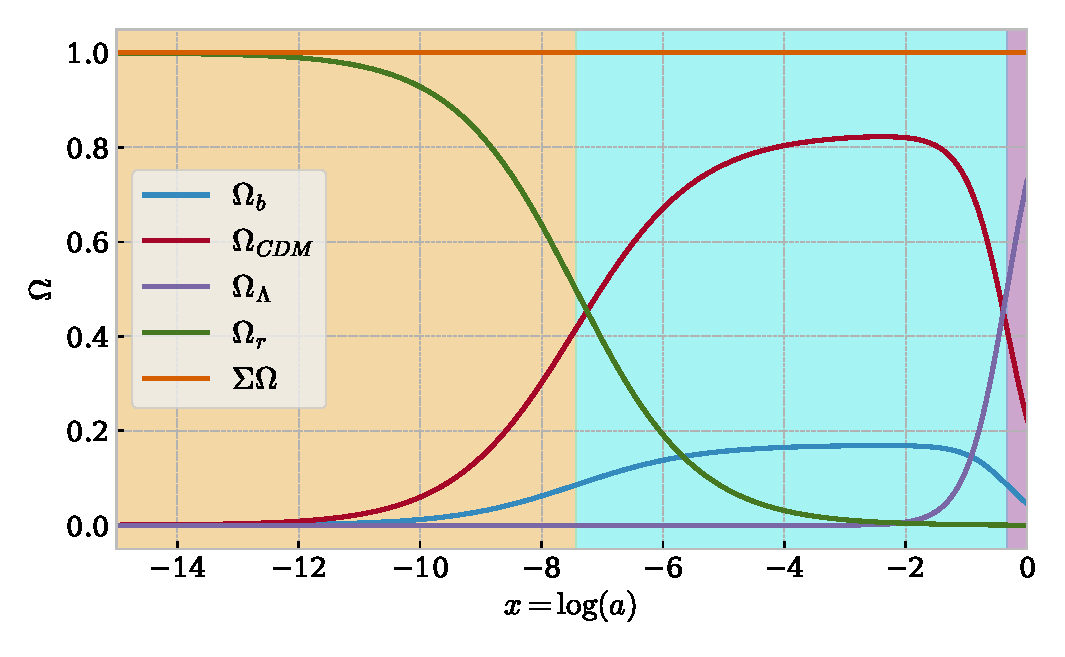
\includegraphics[scale=1]{Figures/Omegas_of_x.pdf}
    \caption{The figure shows the matter-energy density parameters of each component of the total matter-energy content of the universe. Also shown is the sum of all density parameters. To illustrate which component dominates the energy content of the universe at each time, we have colored the radiation domminated era yellow, the matter domminated era blue and the era domminated by dark energy by purple.}
    \label{fig:Omegas}
\end{figure*}

\section{Conclusion} \label{sec:Conclusion}

\bibliography{ref}
\bibliographystyle{aasjournal}
\end{document}

% End of file `sample62.tex'.
